  
\documentclass[tikz,border=5pt]{standalone}
\usetikzlibrary{bending,angles,quotes}
\usepackage{fourier}
\begin{document}

    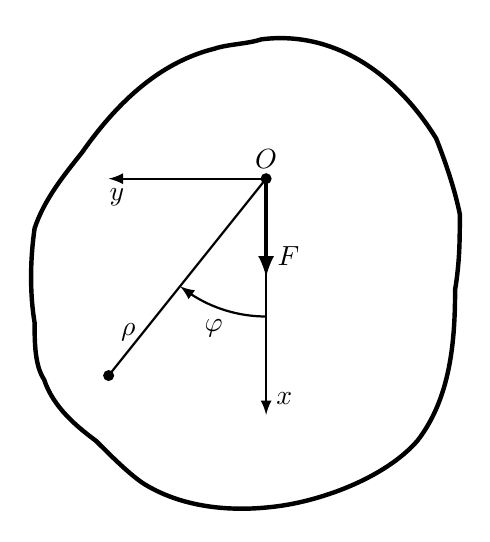
\begin{tikzpicture}
        \begin{scope}[yscale=-1,yshift=-10cm,scale=.6]%<-
          \draw[ultra thick,smooth] (5.4, 0.8).. controls (7.0, 0.6) and (8.3, 1.6) .. (9.1, 2.9).. controls (9.3, 3.4) and (9.5, 4.0) .. (9.6, 4.5).. controls (9.6, 5.0) and (9.6, 5.5) .. (9.5, 6.1).. controls (9.5, 7.2) and (9.4, 8.4) .. (8.7, 9.3).. controls (8.0, 10.1) and (6.6, 10.6) .. (5.6, 10.7).. controls (4.7, 10.8) and (3.7,10.7) .. (2.9, 10.2).. controls (2.6, 10.0) and (2.2, 9.6) .. (1.9, 9.3).. controls (1.5, 9.0) and (1.0, 8.6) .. (0.8, 8.0).. controls (0.6, 7.7) and (0.6, 7.2) .. (0.6, 6.8).. controls (0.5, 6.2) and (0.5, 5.5) .. (0.6, 4.8).. controls (0.8, 4.2) and (1.2, 3.7) .. (1.6, 3.2).. controls (2.3, 2.2) and  (3.2, 1.3) .. (4.4, 1.0).. controls (4.7, 0.9) and (5.1, 0.9) .. (5.4, 0.8);
        \end{scope}
        \begin{scope}[shift={(-1.2,2.25)},thick]
        \fill (4.5,5.5) coordinate (O) circle[radius=2pt] 
              (2.5,3) coordinate (rho) circle[radius=2pt];
        \draw (O) node[above] {$O$} -- node[above,pos=.875] {$\rho$} (rho);
        \draw[-latex] (O) -- ++(-2,0) node[below,xshift=3pt] {$y$};
        \draw[-latex] (O) -- ++(0,-3) coordinate (x-axis) node[above right] {$x$};
        \draw[-latex,ultra thick] (O) -- ++(0,-1.25) node[above right] {$F$};
        \pic[angle radius=1.75cm,angle eccentricity=1.15,"$\varphi$",draw,latex-] {angle= rho--O--x-axis};
        \end{scope}
    \end{tikzpicture}

\end{document}